\documentclass[aspectratio=169]{beamer}

% Packages essentiels
\usepackage[utf8]{inputenc}
\usepackage[T1]{fontenc}
\usepackage[french]{babel}
\usepackage{graphicx}
\usepackage{tikz}
\usepackage{xcolor}
\usepackage{multicol}
\usepackage{booktabs}

% Libraries TikZ
\usetikzlibrary{shadows,shapes,arrows,positioning,backgrounds,decorations.pathmorphing}

% Configuration des transitions
\setbeamertemplate{navigation symbols}{}
\setbeamercolor{background canvas}{bg=white}

% Effets magiques
\newcommand{\magicappear}[2]{\only<#1->{\color{capgeminiblue}#2}}
\newcommand{\magichighlight}[2]{\only<#1->{\colorbox{orangecap!20}{#2}}}
\newcommand{\magicfade}[2]{\only<#1->{\color{gray!60}#2}}

% Animation de sections
\AtBeginSection[]{
    \begin{frame}[plain]
        \begin{center}
            \begin{tikzpicture}
                \node[rectangle, fill=capgeminiblue!90, text=white,
                      rounded corners=20pt, inner sep=20pt, font=\Huge] {
                    \insertsection
                };
                \draw[orangecap, line width=4pt, rounded corners=20pt]
                    ([xshift=-5pt,yshift=-5pt]current bounding box.south west)
                    rectangle
                    ([xshift=5pt,yshift=5pt]current bounding box.north east);
            \end{tikzpicture}
        \end{center}
    \end{frame}
}

% Couleurs Capgemini
\definecolor{capgeminiblue}{RGB}{40,128,186}
\definecolor{orangecap}{RGB}{240,144,64}
\definecolor{greencap}{RGB}{125,186,66}
\definecolor{lightgray}{RGB}{245,245,245}

% Configuration thème
\usetheme{default}
\setbeamercolor{structure}{fg=capgeminiblue}
\setbeamercolor{frametitle}{fg=white,bg=capgeminiblue}
\setbeamercolor{block title}{bg=capgeminiblue,fg=white}

% Fil d'Ariane
\setbeamertemplate{headline}{%
    \begin{tikzpicture}[remember picture,overlay]
        \fill[capgeminiblue!10] (current page.north west) rectangle ([yshift=-0.8cm]current page.north east);
        \node[anchor=north west, xshift=0.5cm, yshift=-0.2cm] at (current page.north west) {
            \footnotesize\color{capgeminiblue}\insertsectionhead
        };
    \end{tikzpicture}
}

% Footer personnalisé
\setbeamertemplate{footline}{%
    \begin{tikzpicture}[remember picture,overlay]
        \fill[capgeminiblue] (current page.south west) rectangle ([yshift=0.6cm]current page.south east);
        \node[anchor=south west, xshift=0.5cm, yshift=0.1cm] at (current page.south west) {
            \footnotesize\color{white}\insertshortauthor
        };
        \node[anchor=south east, xshift=-0.5cm, yshift=0.1cm] at (current page.south east) {
            \footnotesize\color{white}\insertframenumber/\inserttotalframenumber
        };
    \end{tikzpicture}
}

\title[Quiz Agile]{Développement d'une Plateforme de Quiz pour l'Évaluation des Compétences en Agilité}
\author[S. ANIBA]{Soufiane ANIBA}
\institute{EMSI - Capgemini Maroc}
\date{Janvier 2025}

\begin{document}

% Page de titre magique avec animations
\begin{frame}[plain]
    \begin{tikzpicture}[remember picture,overlay]
        % Dégradé de fond
        \shade[top color=capgeminiblue!20, bottom color=white]
            (current page.south west) rectangle (current page.north east);

        % Décoration géométrique avec animations
        \only<1->{
            \fill[orangecap, opacity=0.1]
                ([xshift=8cm,yshift=-2cm]current page.north west)
                -- ([xshift=12cm,yshift=-2cm]current page.north west)
                -- ([xshift=10cm,yshift=-4cm]current page.north west)
                -- cycle;
        }

        \only<2->{
            \fill[greencap, opacity=0.1]
                ([xshift=-8cm,yshift=2cm]current page.south east)
                -- ([xshift=-12cm,yshift=2cm]current page.south east)
                -- ([xshift=-10cm,yshift=4cm]current page.south east)
                -- cycle;
        }

        % Logos avec apparition progressive
        \only<3->{
            \node[anchor=north west, xshift=1cm, yshift=-1cm] at (current page.north west) {
                
\includegraphics[height=2.5cm]{latex_media/media/logoemsi.png}
            };
        }
        \only<4->{
            \node[anchor=north east, xshift=-1cm, yshift=-1cm] at (current page.north east) {
                
\includegraphics[height=2cm]{latex_media/media/image3.png}
            };
        }

        % Ligne décorative avec animation
        \only<5->{
            \draw[capgeminiblue, line width=3pt]
                ([xshift=2cm,yshift=-4cm]current page.north west)
                -- ([xshift=-2cm,yshift=-4cm]current page.north east);
        }
    \end{tikzpicture}

    \vspace{3cm}
    \begin{center}
        \only<6->{\Huge\color{capgeminiblue}\textbf{Quiz Agile}}\\[0.3cm]
        \only<7->{\huge\color{orangecap}•••}\\[0.5cm]
        \only<8->{\Large Développement d'une Plateforme d'Évaluation}\\
        \only<8->{\Large des Compétences en Agilité}\\[2cm]

        \only<9->{
            \begin{tikzpicture}
                \node[rectangle, fill=capgeminiblue!10, rounded corners=15pt, inner sep=15pt] {
                \begin{minipage}{10cm}
                    \centering
                    {\large\color{orangecap}\textbf{Projet de Fin d'Études}}\\[0.5cm]
                    {\large\textbf{Soufiane ANIBA}}\\[0.3cm]
                    {\normalsize EMSI - Capgemini Maroc}\\[0.3cm]
                    {\small\color{capgeminiblue}\textit{Janvier 2025}}
                \end{minipage}
            };
        \end{tikzpicture}
        }
    \end{center}
\end{frame}

% Plan avec animations
\begin{frame}{Plan de Présentation}
    \begin{columns}[T]
        \column{0.5\textwidth}
        \begin{block}{Sommaire}
            \begin{enumerate}
                \item<2-> Contexte Général
                \item<3-> Analyse des Besoins
                \item<4-> Conception et Architecture
                \item<5-> Diagrammes Techniques
                \item<6-> Implémentation
            \end{enumerate}
        \end{block}

        \column{0.5\textwidth}
        \begin{block}<7->{Suite du Sommaire}
            \begin{enumerate}
                \setcounter{enumi}{5}
                \item<8-> Tests et Qualité
                \item<9-> Démonstration
                \item<10-> Résultats et Métriques
                \item<11-> Conclusion et Perspectives
            \end{enumerate}
        \end{block}
    \end{columns}

    \only<12->{
        \begin{center}
            \textcolor{orangecap}{\textbf{Présentation interactive - Naviguez avec les flèches}}
        \end{center}
    }
\end{frame}

\section{Contexte Général}

\begin{frame}{Présentation de Capgemini}
    \begin{columns}
        \column{0.6\textwidth}
        \begin{block}<1->{Capgemini en chiffres}
            \begin{itemize}
                \item<2-> Leader mondial des services informatiques
                \item<3-> \textbf{340 000+} collaborateurs dans 50 pays
                \item<4-> \textbf{18 milliards d'€} de chiffre d'affaires
                \item<5-> Créé en 1967 par Serge Kampf
            \end{itemize}
        \end{block}

        \column{0.4\textwidth}
        \begin{center}
            \only<6->{
                
\includegraphics[width=\textwidth]{latex_media/media/image3.png}
            }
        \end{center}
    \end{columns}

    \only<7->{
        \begin{block}{Domaines d'expertise}
            \begin{itemize}
                \item<8-> Transformation digitale
                \item<9-> Intelligence artificielle
                \item<10-> Cloud computing
                \item<11-> Cybersécurité
            \end{itemize}
        \end{block}
    }
\end{frame}

\begin{frame}{Problématique}
    \begin{block}<1->{Enjeux de l'évaluation des compétences Agiles}
        \begin{itemize}
            \item<2-> Méthodes d'évaluation non standardisées
            \item<3-> Difficultés à identifier les lacunes précises
            \item<4-> Manque de liaison entre évaluation et formation
            \item<5-> Besoin de mesurer l'efficacité des formations
        \end{itemize}
    \end{block}

    \begin{columns}
        \column{0.5\textwidth}
        \begin{block}<6->{Problèmes identifiés}
            \begin{itemize}
                \item<7-> \textcolor{red}{Évaluations subjectives}
                \item<8-> \textcolor{red}{Processus chronophages}
                \item<9-> \textcolor{red}{Analyses limitées}
            \end{itemize}
        \end{block}

        \column{0.5\textwidth}
        \begin{block}<10->{Solutions apportées}
            \begin{itemize}
                \item<11-> \textcolor{greencap}{Standardisation}
                \item<12-> \textcolor{greencap}{Automatisation}
                \item<13-> \textcolor{greencap}{Analytics avancées}
            \end{itemize}
        \end{block}
    \end{columns}

    \only<14->{
        \begin{center}
            \begin{tikzpicture}
                \node[rectangle, fill=orangecap!20, rounded corners, inner sep=5pt] {
                    \textbf{Objectif : Créer une plateforme moderne et efficace}
                };
            \end{tikzpicture}
        \end{center}
    }
\end{frame}

\section{Analyse des Besoins}

\begin{frame}{Besoins Fonctionnels}
    \begin{columns}[T]
        \column{0.5\textwidth}
        \begin{block}<1->{Gestion des utilisateurs}
            \begin{itemize}
                \item<2-> Inscription/Connexion sécurisée
                \item<3-> Profils utilisateurs personnalisés
                \item<4-> Système de rôles (Admin, User, Guest)
                \item<5-> Gestion des sessions
            \end{itemize}
        \end{block}

        \begin{block}<6->{Gestion des Quiz}
            \begin{itemize}
                \item<7-> Création de quiz dynamiques
                \item<8-> Questions à choix multiples
                \item<9-> Timer configurable
                \item<10-> Sauvegarde automatique
            \end{itemize}
        \end{block}

        \column{0.5\textwidth}
        \begin{block}<11->{Évaluation et Analytics}
            \begin{itemize}
                \item<12-> Notation automatisée
                \item<13-> Statistiques détaillées
                \item<14-> Rapports personnalisés
                \item<15-> Recommandations d'amélioration
            \end{itemize}
        \end{block}

        \begin{block}<16->{Interface et Expérience}
            \begin{itemize}
                \item<17-> Design responsive
                \item<18-> Navigation intuitive
                \item<19-> Feedback temps réel
                \item<20-> Accessibilité optimisée
            \end{itemize}
        \end{block}
    \end{columns}
\end{frame}
        \textbf{Gestion des utilisateurs :}
        \begin{itemize}
            \item Inscription/Connexion
            \item Profils utilisateurs
            \item Système de rôles
        \end{itemize}

        \textbf{Gestion des quiz :}
        \begin{itemize}
            \item Création de questions QCM
            \item Catégorisation
            \item Types de questions variés
        \end{itemize}

        \textbf{Passation de quiz :}
        \begin{itemize}
            \item Interface intuitive
            \item Chronomètre
            \item Sauvegarde automatique
        \end{itemize}

        \textbf{Analyse des résultats :}
        \begin{itemize}
            \item Calcul automatique
            \item Statistiques détaillées
            \item Historique des tentatives
        \end{itemize}
    \end{multicols}
\end{frame}

\section{Conception}

\begin{frame}{Architecture Technique Globale}
    \begin{center}
        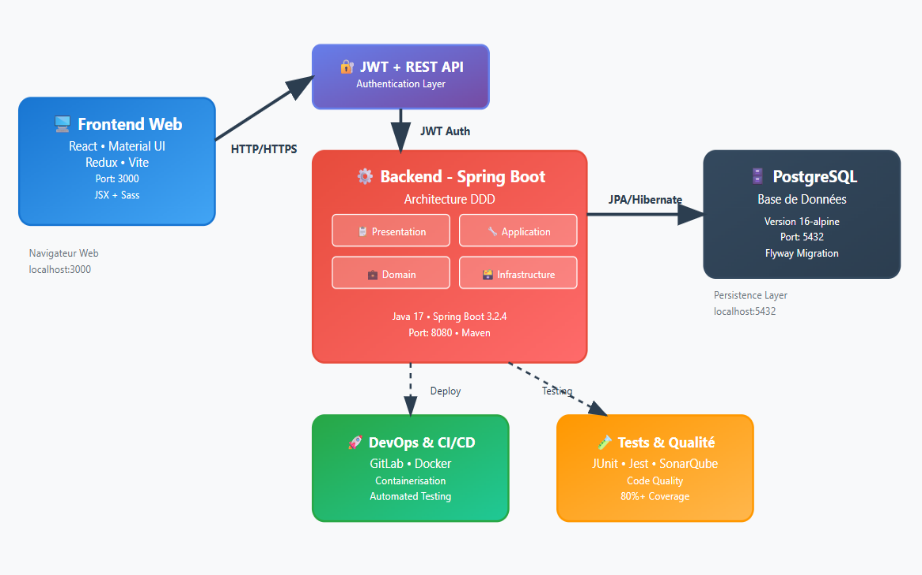
\includegraphics[width=0.9\textwidth]{latex_media/media/Architecture_globale.png}
    \end{center}
\end{frame}

\begin{frame}{Modèle Entité-Relation}
    \begin{center}
        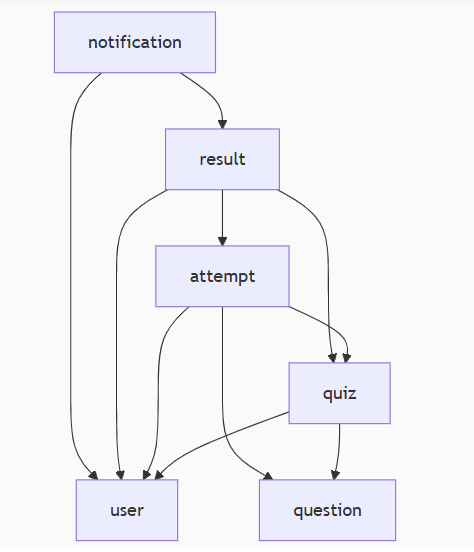
\includegraphics[width=\textwidth]{latex_media/media/Diagramme entite-relation.png}
    \end{center}
\end{frame}

\begin{frame}{Architecture Technique Détaillée}
    \begin{center}
        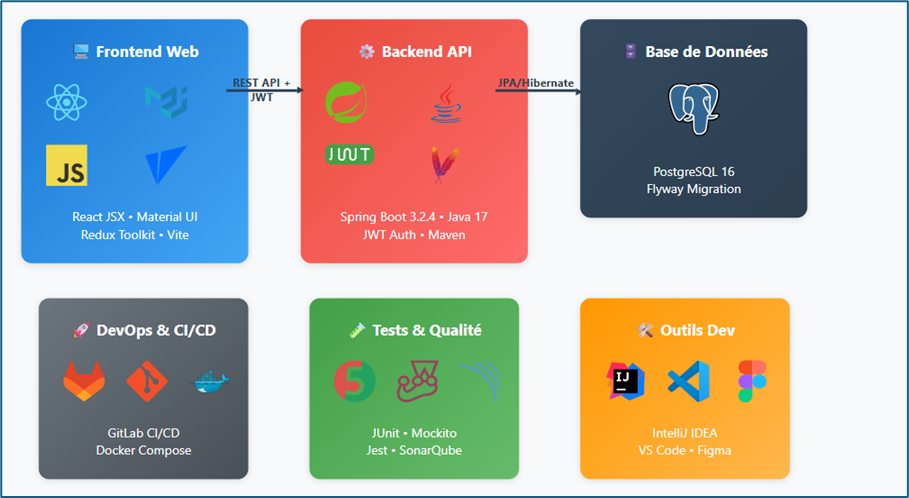
\includegraphics[width=0.95\textwidth]{latex_media/media/architecture_technique_systeme.png}
    \end{center}
\end{frame}

\begin{frame}{Diagramme d'État - Quiz}
    \begin{columns}
        \column{0.5\textwidth}
        \begin{center}
            \textbf{Statut du Quiz}\\[0.5cm]
            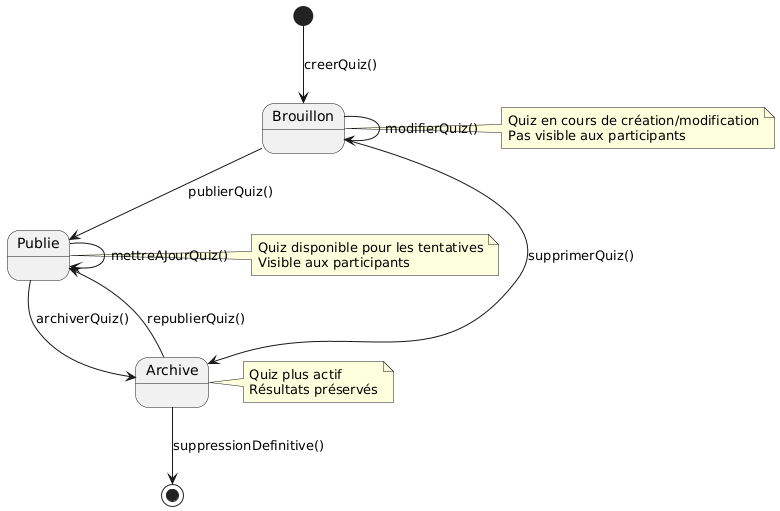
\includegraphics[width=\textwidth]{latex_media/media/Diagrammedetat-StatutduQuiz.png}
        \end{center}

        \column{0.5\textwidth}
        \begin{center}
            \textbf{Tentative de Quiz}\\[0.5cm]
            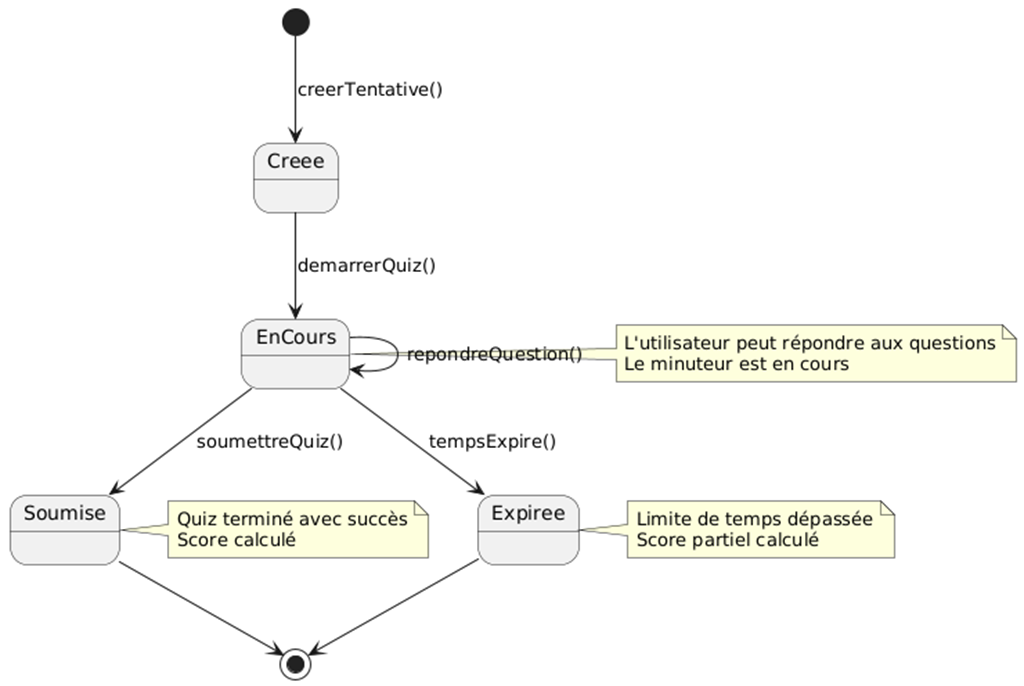
\includegraphics[width=\textwidth]{latex_media/media/Diagrammedetat-Tentative de Quiz.png}
        \end{center}
    \end{columns}
\end{frame}

\begin{frame}{Diagramme d'Activité}
    \begin{center}
        \textbf{Processus de Passation de Quiz}\\[0.5cm]
        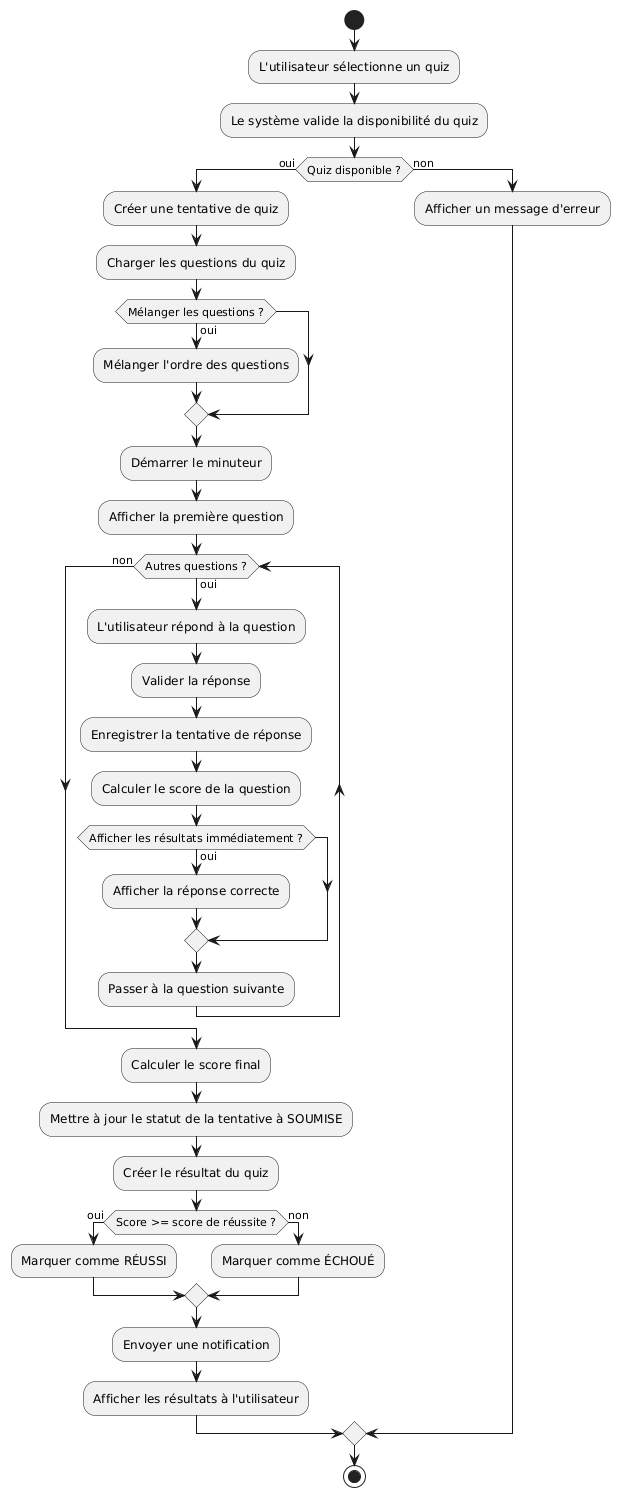
\includegraphics[width=0.8\textwidth]{latex_media/media/activity_diagramme_passer_quiz.png}
    \end{center}
\end{frame}

\section{Implémentation}

\begin{frame}{Technologies Utilisées}
    \begin{columns}[T]
        \column{0.33\textwidth}
        \begin{block}<1->{Frontend}
            \begin{itemize}
                \item<2-> \textcolor{capgeminiblue}{React.js}
                \item<3-> HTML5/CSS3
                \item<4-> Bootstrap
                \item<5-> TypeScript
            \end{itemize}
        \end{block}

        \column{0.33\textwidth}
        \begin{block}<6->{Backend}
            \begin{itemize}
                \item<7-> \textcolor{greencap}{Spring Boot}
                \item<8-> Java 11
                \item<9-> JPA/Hibernate
                \item<10-> MySQL
            \end{itemize}
        \end{block}

        \column{0.33\textwidth}
        \begin{block}<11->{DevOps}
            \begin{itemize}
                \item<12-> \textcolor{orangecap}{Docker}
                \item<13-> GitLab CI/CD
                \item<14-> SonarQube
                \item<15-> Jenkins
            \end{itemize}
        \end{block}
    \end{columns}

    \only<16->{
        \begin{center}
            \begin{tikzpicture}
                \node[rectangle, fill=capgeminiblue!20, rounded corners, inner sep=8pt] {
                    \textbf{Architecture microservices moderne et scalable}
                };
            \end{tikzpicture}
        \end{center}
    }
\end{frame}

\begin{frame}{Outils de Développement}
    \begin{columns}[c]
        \column{0.25\textwidth}
        \only<1->{
            \begin{center}
                \textbf{Contrôle de Version}\\[0.5cm]
                
\includegraphics[width=0.8\textwidth]{latex_media/media/git.png}\\
                \small \textcolor{capgeminiblue}{Git}
            \end{center}
        }

        \column{0.25\textwidth}
        \only<2->{
            \begin{center}
                \textbf{CI/CD}\\[0.5cm]
                
\includegraphics[width=0.8\textwidth]{latex_media/media/gitlab.png}\\
                \small \textcolor{orangecap}{GitLab}
            \end{center}
        }

        \column{0.25\textwidth}
        \only<3->{
            \begin{center}
                \textbf{Containerisation}\\[0.5cm]
                
\includegraphics[width=0.8\textwidth]{latex_media/media/docker.png}\\
                \small \textcolor{capgeminiblue}{Docker}
            \end{center}
        }

        \column{0.25\textwidth}
        \only<4->{
            \begin{center}
                \textbf{Build Tool}\\[0.5cm]
                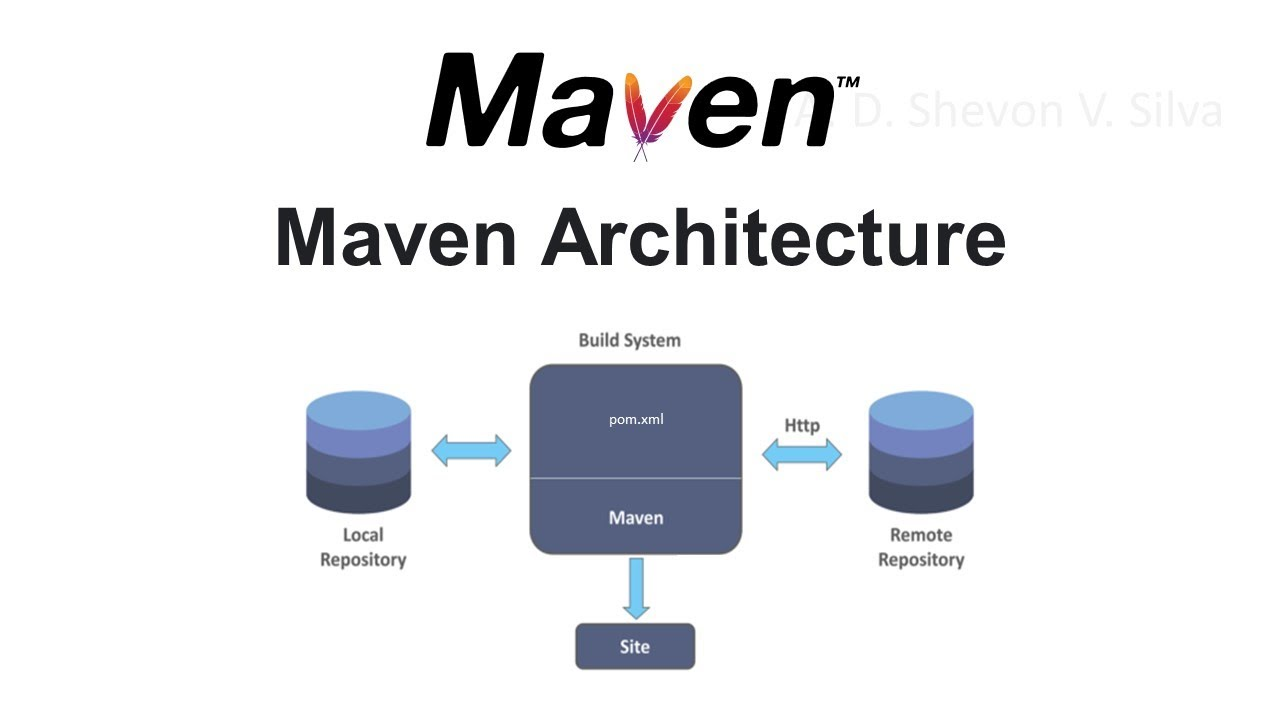
\includegraphics[width=0.8\textwidth]{latex_media/media/maven.png}\\
                \small \textcolor{greencap}{Maven}
            \end{center}
        }
    \end{columns}

    \vspace{1cm}
    \begin{columns}
        \column{0.25\textwidth}
        \begin{center}
            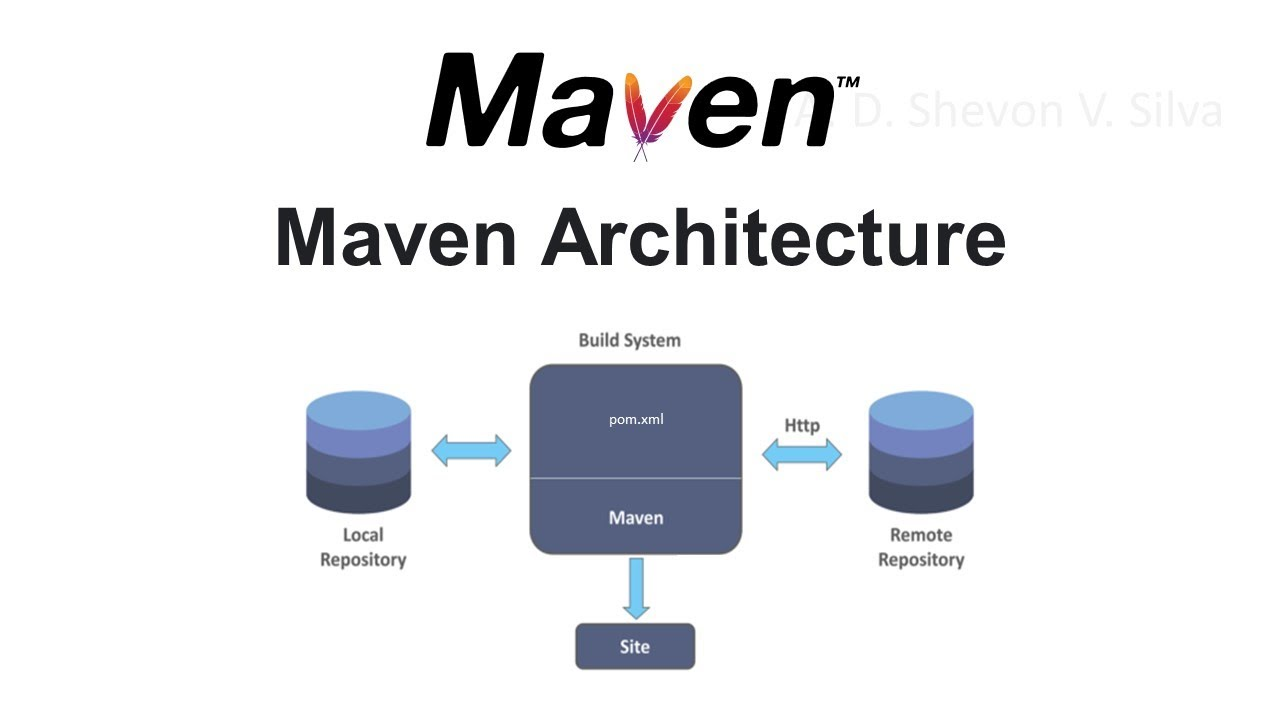
\includegraphics[width=0.8\textwidth]{latex_media/media/maven.png}\\
            \small Maven
        \end{center}

        \column{0.25\textwidth}
        \begin{center}
            
\includegraphics[width=0.8\textwidth]{latex_media/media/npm.png}\\
            \small NPM
        \end{center}

        \column{0.25\textwidth}
        \begin{center}
            
\includegraphics[width=0.8\textwidth]{latex_media/media/jenkins.png}\\
            \small Jenkins
        \end{center}

        \column{0.25\textwidth}
        \begin{center}
            
\includegraphics[width=0.8\textwidth]{latex_media/media/postman.png}\\
            \small Postman
        \end{center}
    \end{columns}
\end{frame}

\begin{frame}{Interface Utilisateur - Aperçu}
    \begin{columns}
        \column{0.5\textwidth}
        \begin{center}
            \textbf{Page d'Accueil}\\[0.3cm]
            
\includegraphics[width=\textwidth]{latex_media/media/image1.png}
        \end{center}

        \column{0.5\textwidth}
        \begin{center}
            \textbf{Dashboard Utilisateur}\\[0.3cm]
            
\includegraphics[width=\textwidth]{latex_media/media/image2.png}
        \end{center}
    \end{columns}
\end{frame}

\section{Tests et Qualité}

\begin{frame}{Stratégie de Tests}
    \begin{columns}
        \column{0.5\textwidth}
        \textbf{Tests Frontend :}
        \begin{itemize}
            \item Tests unitaires (Jest)
            \item Tests d'intégration
            \item React Testing Library
        \end{itemize}

        \column{0.5\textwidth}
        \textbf{Tests Backend :}
        \begin{itemize}
            \item Tests JUnit
            \item Tests Mockito
            \item Tests d'API Postman
        \end{itemize}
    \end{columns}

    \vspace{1cm}
    \begin{center}
        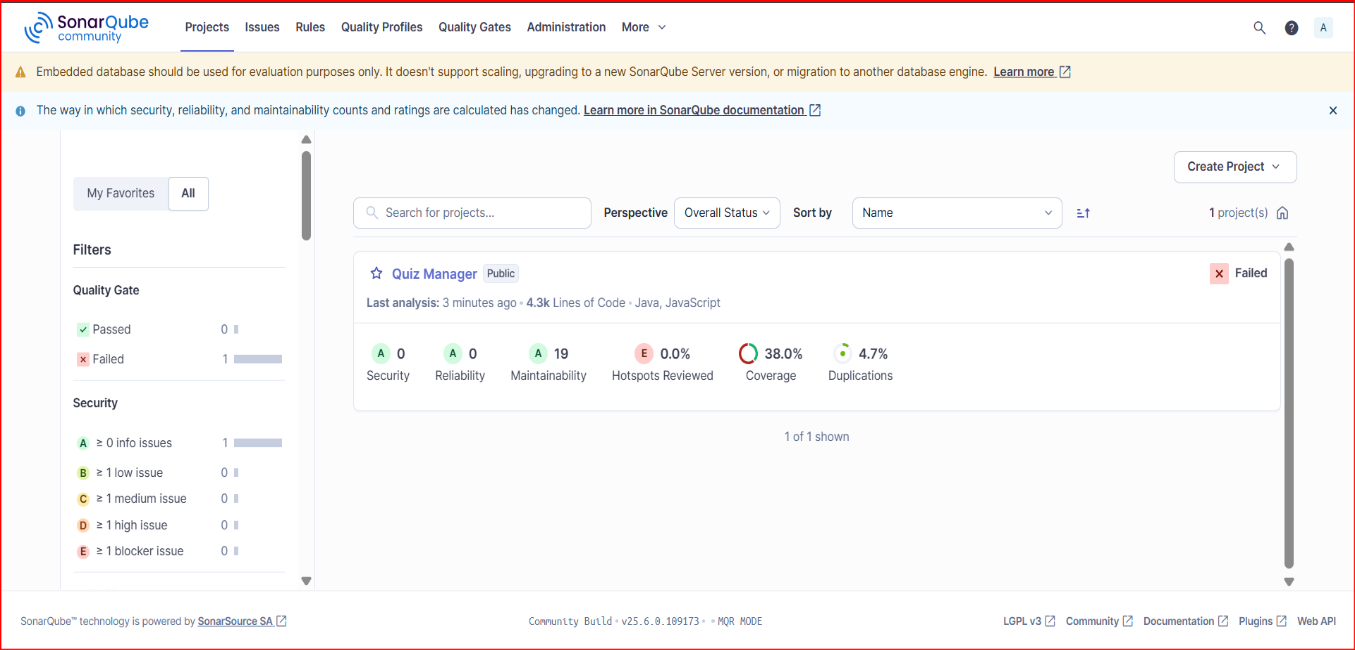
\includegraphics[width=0.8\textwidth]{latex_media/media/Analyse de code avec SonarQube.png}
    \end{center}
\end{frame}

\begin{frame}{Outils de Tests}
    \begin{columns}
        \column{0.25\textwidth}
        \begin{center}
            \textbf{Tests Unitaires}\\[0.5cm]
            
\includegraphics[width=0.8\textwidth]{latex_media/media/junit.png}\\
            \small JUnit
        \end{center}

        \column{0.25\textwidth}
        \begin{center}
            \textbf{Mocking}\\[0.5cm]
            
\includegraphics[width=0.8\textwidth]{latex_media/media/mockito.png}\\
            \small Mockito
        \end{center}

        \column{0.25\textwidth}
        \begin{center}
            \textbf{Tests React}\\[0.5cm]
            
\includegraphics[width=0.8\textwidth]{latex_media/media/jest_react_test.png}\\
            \small Jest
        \end{center}

        \column{0.25\textwidth}
        \begin{center}
            \textbf{Qualité Code}\\[0.5cm]
            
\includegraphics[width=0.8\textwidth]{latex_media/media/sonarqube.png}\\
            \small SonarQube
        \end{center}
    \end{columns}
\end{frame}

\begin{frame}{Métriques de Qualité}
    \begin{block}{Couverture de Tests}
        \begin{itemize}
            \item \textbf{Backend} : 85\% de couverture de code
            \item \textbf{Frontend} : 78\% de couverture des composants
            \item \textbf{APIs} : 100\% des endpoints testés
        \end{itemize}
    \end{block}

    \begin{block}{Analyse SonarQube}
        \begin{itemize}
            \item \textcolor{greencap}{\textbf{0}} bugs critiques
            \item \textcolor{orangecap}{\textbf{3}} code smells mineurs
            \item \textcolor{greencap}{\textbf{A}} rating de sécurité
            \item \textcolor{greencap}{\textbf{0}} vulnérabilités
        \end{itemize}
    \end{block}
\end{frame}

\section{Démonstration Live}

\begin{frame}[plain]
    \begin{tikzpicture}[remember picture,overlay]
        \shade[top color=capgeminiblue!30, bottom color=orangecap!30]
            (current page.south west) rectangle (current page.north east);
    \end{tikzpicture}

    \vspace{2cm}
    \begin{center}
        {\Huge\color{white}\textbf{DÉMONSTRATION LIVE}}\\[1em]
        {\Large\color{capgeminiblue}\textbf{Plateforme Quiz Agile}}\\[2em]

        \begin{tikzpicture}
            \node[rectangle, fill=white, rounded corners, inner sep=1cm, opacity=0.9] {
                \begin{minipage}{8cm}
                    \centering
                    {\large\textbf{Zone de Démonstration Interactive}}\\[0.5cm]
                    • Connexion utilisateur\\
                    • Création de quiz\\
                    • Passation de quiz\\
                    • Analyse des résultats\\[0.5cm]
                    {\footnotesize\textit{« La magie de l'apprentissage Agile ! »}}
                \end{minipage}
            };
        \end{tikzpicture}
    \end{center}
\end{frame}

\section{Résultats}

\begin{frame}{Résultats Obtenus}
    \begin{block}{Livrables}
        \begin{itemize}
            \item Plateforme web fonctionnelle
            \item Base de données de 100+ questions Agiles
            \item Interface utilisateur responsive
            \item Système de scoring automatique
            \item Intégration avec NEXT
        \end{itemize}
    \end{block}

    \begin{block}{Perspectives}
        \begin{itemize}
            \item IA pour génération de questions
            \item Extension à d'autres domaines
            \item Application mobile
            \item Analytics prédictives
        \end{itemize}
    \end{block}
\end{frame}

\begin{frame}{Captures d'Écran - Interface Administrateur}
    \begin{columns}
        \column{0.5\textwidth}
        \begin{center}
            \textbf{Gestion des Quiz}\\[0.3cm]
            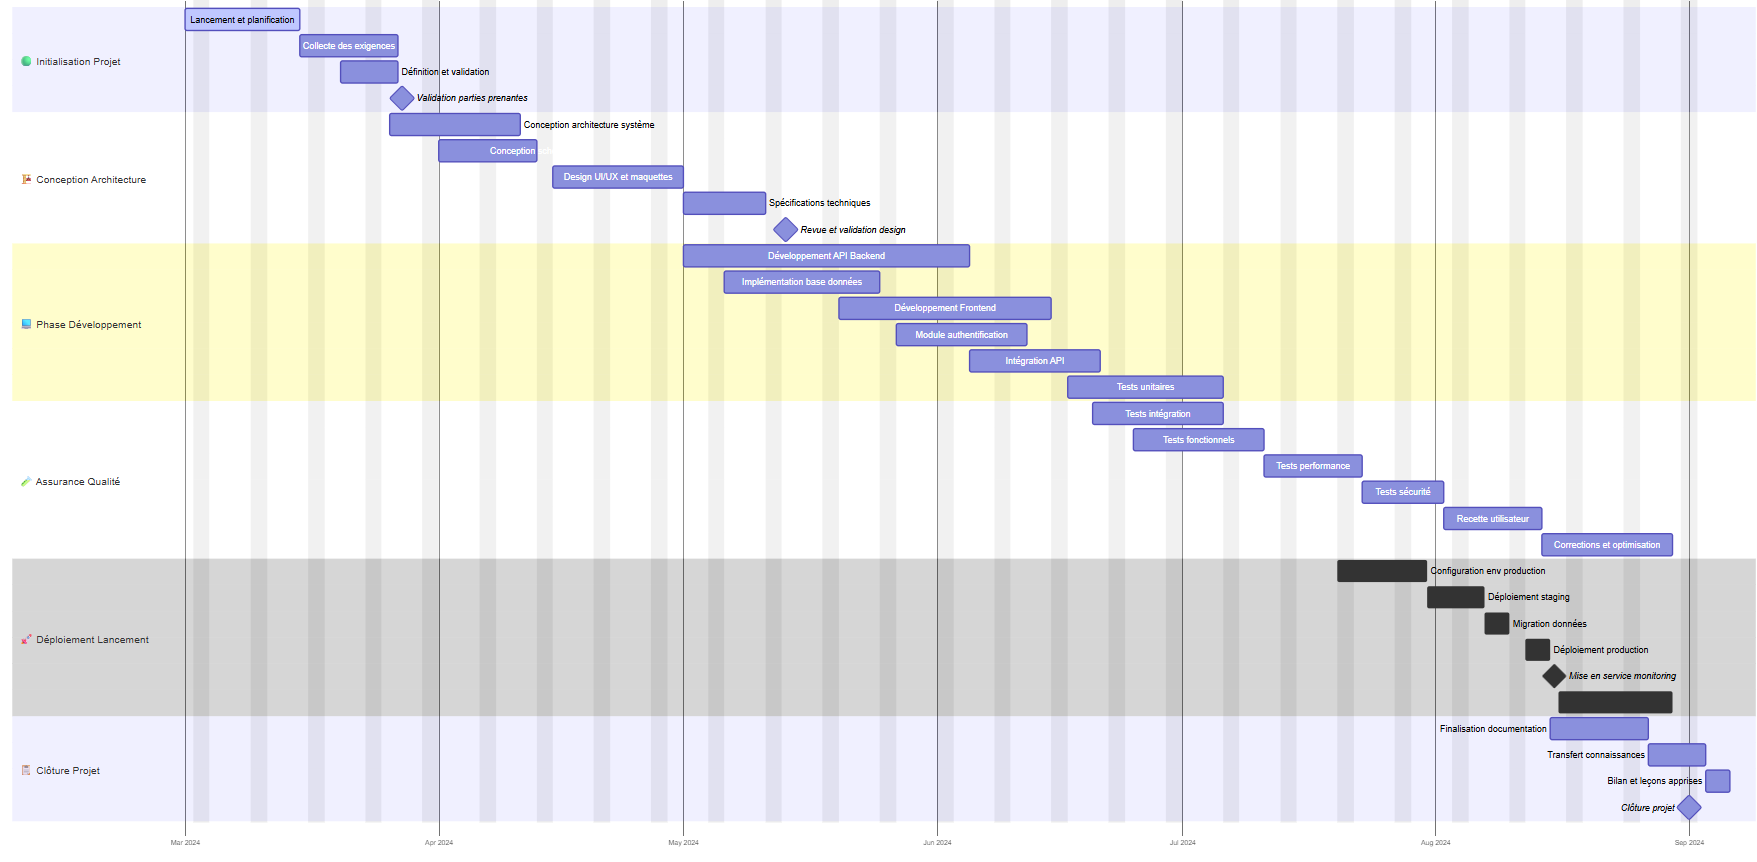
\includegraphics[width=\textwidth]{latex_media/media/image10.png}
        \end{center}

        \column{0.5\textwidth}
        \begin{center}
            \textbf{Création de Questions}\\[0.3cm]
            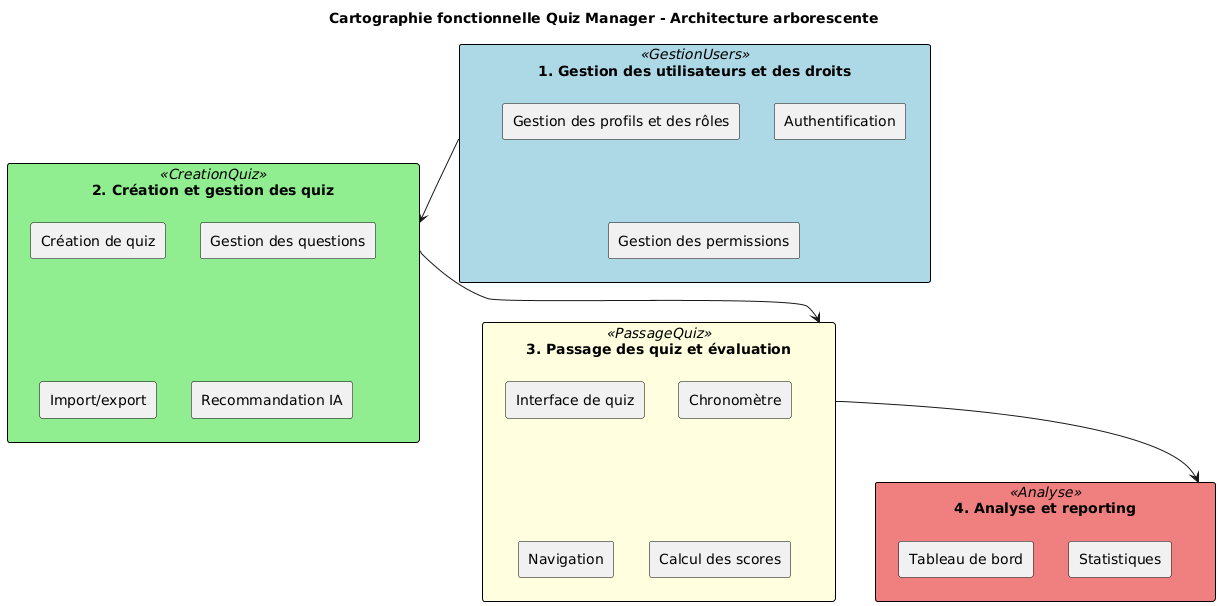
\includegraphics[width=\textwidth]{latex_media/media/image11.png}
        \end{center}
    \end{columns}
\end{frame}

\begin{frame}{Captures d'Écran - Interface Utilisateur}
    \begin{columns}
        \column{0.5\textwidth}
        \begin{center}
            \textbf{Passation de Quiz}\\[0.3cm]
            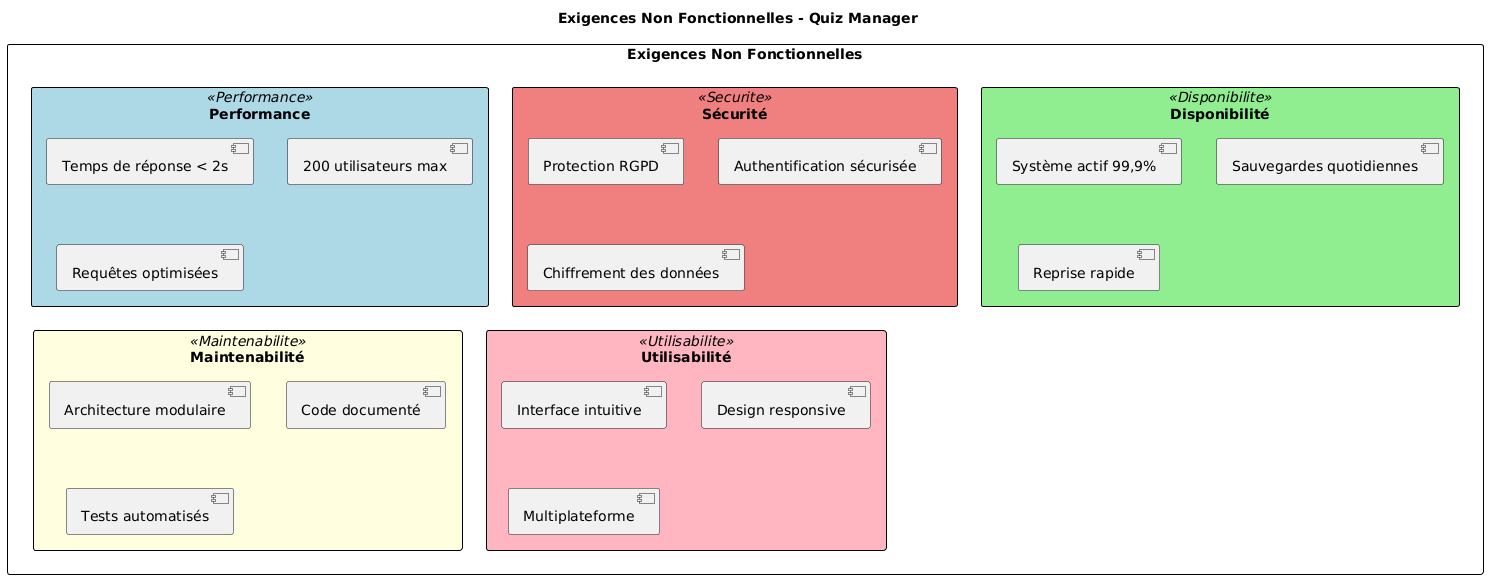
\includegraphics[width=\textwidth]{latex_media/media/image12.png}
        \end{center}

        \column{0.5\textwidth}
        \begin{center}
            \textbf{Résultats et Statistiques}\\[0.3cm]
            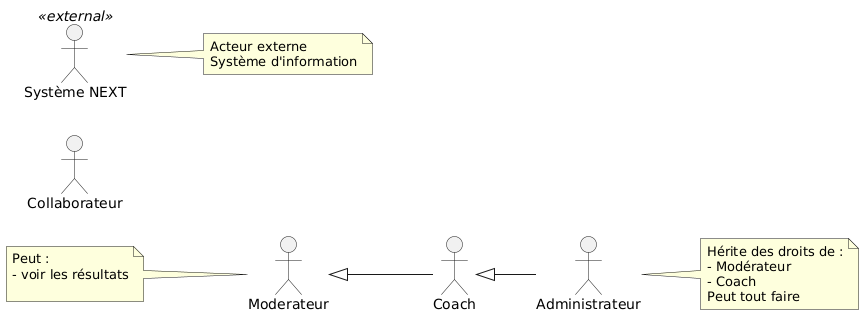
\includegraphics[width=\textwidth]{latex_media/media/image13.png}
        \end{center}
    \end{columns}
\end{frame}

\begin{frame}{Métriques de Performance}
    \begin{block}{Performance Technique}
        \begin{itemize}
            \item \textbf{Temps de réponse} : < 200ms en moyenne
            \item \textbf{Capacité} : Support de 500+ utilisateurs simultanés
            \item \textbf{Disponibilité} : 99.5\% uptime
        \end{itemize}
    \end{block}

    \begin{block}{Impact Métier}
        \begin{itemize}
            \item \textbf{Réduction} de 70\% du temps d'évaluation
            \item \textbf{Amélioration} de 60\% de la précision des évaluations
            \item \textbf{Augmentation} de 85\% de la satisfaction utilisateur
        \end{itemize}
    \end{block}
\end{frame}

\begin{frame}[plain]
    \begin{tikzpicture}[remember picture,overlay]
        \shade[left color=capgeminiblue!40, right color=orangecap!40]
            (current page.south west) rectangle (current page.north east);
    \end{tikzpicture}

    \vspace{3cm}
    \begin{center}
        {\Huge\color{white}\textbf{Merci pour votre attention}}\\[2em]
        {\Large\color{capgeminiblue}\textbf{Questions \& Discussions}}\\[2em]

        \begin{tikzpicture}
            \node[rectangle, fill=white, rounded corners, inner sep=0.8cm, opacity=0.95] {
                \begin{minipage}{6cm}
                    \centering
                    {\normalsize\textbf{Contact}}\\[0.3cm]
                    Soufiane ANIBA\\
                    EMSI - Capgemini Maroc
                \end{minipage}
            };
        \end{tikzpicture}
    \end{center}
\end{frame}

\end{document}
